\documentclass[../DefinizioneDiProdotto.tex]{subfiles}
\begin{document}

\section{Diagrammi di sequenza}

	In questa sezione vengono descritte e rappresentate tramite diagrammi di sequenza UML le sequenze di azioni ritenute più significative con lo scopo di facilitare la comprensione delle comunicazioni tra oggetti facenti parte dell'applicativo Android\g\. 
	
	\subsection{Avvio Service per il rilevamento beacon}
		Il diagramma in figura \ref{StartService} rappresenta l'avvio del Service che si occupa del rilevamento dei beacon\g\, funzionalità focale dell'intero applicativo.
	Il PRESENTER chiama \verb|startService()| su un riferimento di tipo \verb|AbsBeaconReceiver|, all'interno del metodo quindi verrà istanziato un oggetto \verb|intent| di tipo \verb|Intent| necessario per creare effettivamente un service unbind di tipo \verb|BeaconManagerAdapter| attraverso la chiamata del metodo \verb|bindService()|,  passando come parametro \verb|intente| creato precedentemente. Nella fase di creazione di \verb|BeaconManagerAdapter| viene chiamato il metodo \verb|onCreate()| nel quale viene creata un istanza della classe \verb|BeaconManager| offerta dalla libreria AltBeacon. Si effettuano inoltre diverse chiamate per il settaggio e la configurazione di \verb|beaconManager| che non sono rappresentate per mantenere il diagramma più leggibile. Una volta settato \verb|beaconManager| l'oggetto \verb|beaconManagerAdapter| si mette in ascolto di \verb|beaconManager| chiamando il metodo \verb|setMonitorNotifier| iniziando la fase di monitoring\g\.
	A questo punto \verb|beaconManagerAdapter| è un listener di \verb|beaconManager| il quale una volta rilevata la region\g\ dei beacon in cui il device si trova scatena l'evento \verb|didEnterRegion()| notificando i propri listener, ossia \verb|beaconManagerAdapter|.
	Individuata la region\g\ tramite l'evento \verb|beaconManagerAdapter| effettua un controllo per capire se la region\g\ è riconosciuta e se lo è \verb|beaconManagerAdapter| entra nella fase di ranging\g\ in cui saranno raccolti dettagliatamente i dati di tutti i beacon rilevati. \verb|beaconManagerAdapter| si mette in ascolto in modalità ranging di \verb|beaconManager| tramite la chiamata del metodo \verb|setRangeNotifier()|.
	A questo punto \verb|beaconManagerAdapter| riceve l'evento di rilevazione beacon attraverso il metodo \verb|didRangeBeaconsInRegion()| il quale restituisce una \verb|Collection| di \verb|Beacon| e la region\g\ di appartenenza.
	Per la gestione degli \verb|Collection| si rimanda al diagramma successivo.
	
		\begin{figure}
			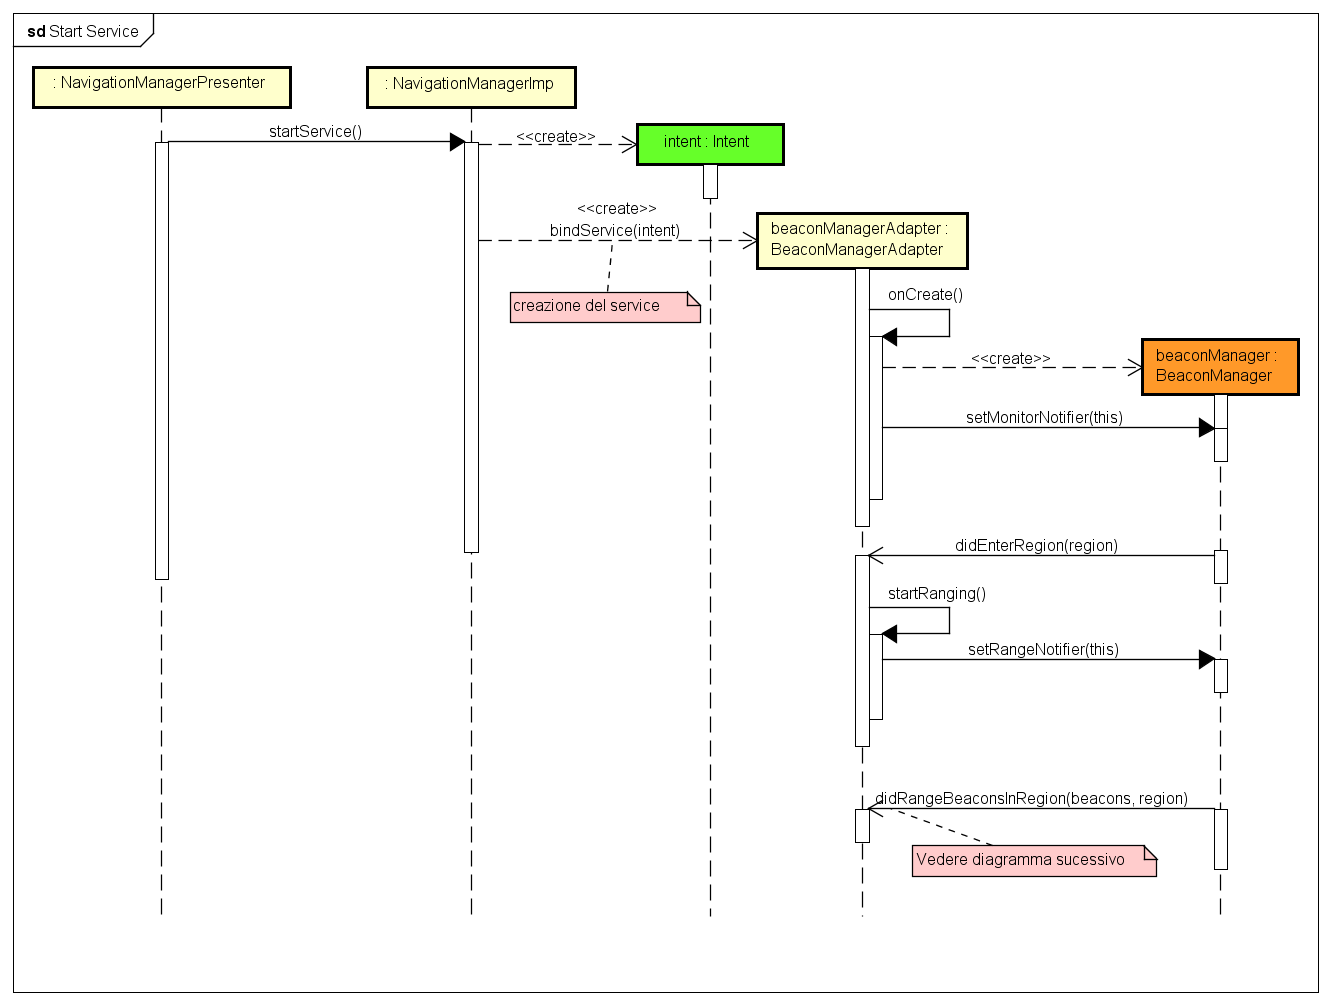
\includegraphics[width=\textwidth]{diagrams/StartService}
			\caption{Diagramma di sequenza - Avvio di un Service per il rilevamento beacon}
			\label{StartService}
		\end{figure}
		
	\subsection{Elaborazione beacon rilevati e comunicazione Broadcast}
		
		
\end{document}